\chapter{Graphing}
\setcounter{figure}{0}
\setcounter{table}{0}
\label{sec:Graphing}

The OptimumTire plotting tool is a powerful feature that allows users to create nearly any type of tire graph that they please. Two different types of graphs can be created in OptimumTire. One is a \textsl{standard graph} which allows plotting of any quantity against any other quantity in either two- or three-dimensions. The other is a \textsl{report graph} which shows measured quantities versus sample number. It is only capable of plotting raw data.

\section{Standard Graphs}
\label{sec:StandardGraphs}
Standard graphs can display raw data and tire models. The data or model to be graphed can be specified by selecting the checkbox next to the desired items in the project tree. A new standard graph can be added to a worksheet in multiple ways. Right clicking on the worksheet or worksheet tabs and selecting \textsl{Add Graph}, selecting \textsl{Add Graph To Worksheet} from the \textsl{Worksheet} menu on the main toolbar or by clicking on the \textsl{Add Graph} button in the toolbar next to the Save button. Up to four graphs can be placed on a single worksheet. When a graph is added to the worksheet the graph setup form will appear in the data entry area. To show the graph setup form when the data entry area is showing another form, click on the graph. You must specify six graph inputs and two or three graph outputs to create a graph. These will be further discussed in the following sections. 

\subsection{Types of Standard Graphs}
\label{sec:TypesofStandardGraphs}
There are three types of standard graphs. Single direction line graphs, crossed line graphs and surface graphs. You can select the type of graph by choosing the appropriate option in the list of radio buttons near the bottom of the data entry form. 

\subsection*{Single Direction Line Graphs}
An example of a single direction line graph is shown in Figure~\ref{fig:SingleDirectionLines}. When plotting models using this type of graph, lines are generated based on the first of the graph inputs. For example, if the first graph input (labeled as \textsl{Indep. Variable}) is slip angle, lines will be generated by varying the slip angle while keeping all the other graph inputs constant.

\begin{figure}[H]
	\centering
		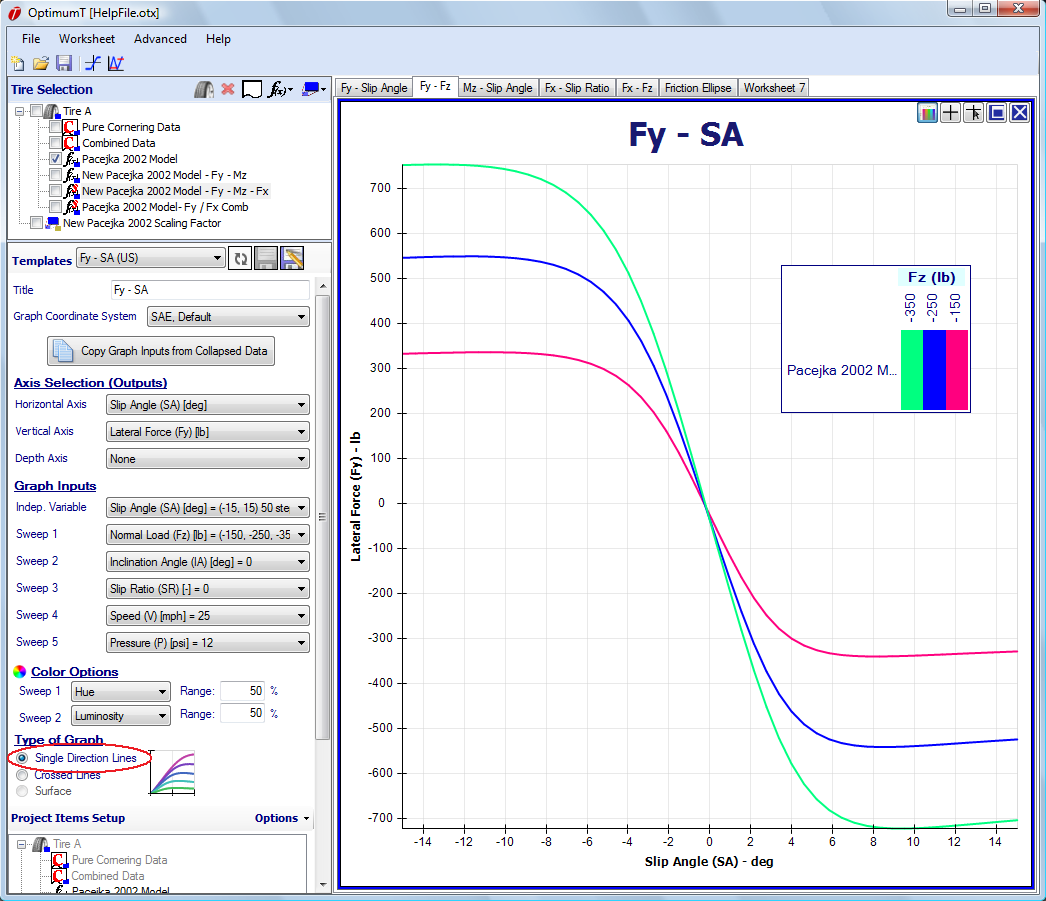
\includegraphics[width=1.0\textwidth]{SingleDirectionLines.png}
	\caption{Single Direction Line Graph}
	\label{fig:SingleDirectionLines}
\end{figure}

\subsection*{Crossed Line Graphs}
An example of a crossed line graph is shown in Figure~\ref{fig:CrossedLineGraph}. As can be seen in the figure there are two independent variables for this type of graph.  Therefore, two sets of lines will be generated for this graph. The first set of lines is generated by varying the first graph input while holding all others constant. The second set of lines is generated by varying the second graph input while holding all the others constant. For example, if the first graph input (labeled \textsl{First Indep.}) is set as slip angle and the second input (labeled \textsl{Second Indep.}) is set as slip ratio, then one set of lines will be generated with constant slip ratio and varying slip angle and another set of lines will be generated with constant slip angle and varying slip ratio. This type of graph is useful when creating a friction ellipse where you want lines of constant slip angle and lines of constant slip ratio.

\begin{figure}[H]
	\centering
		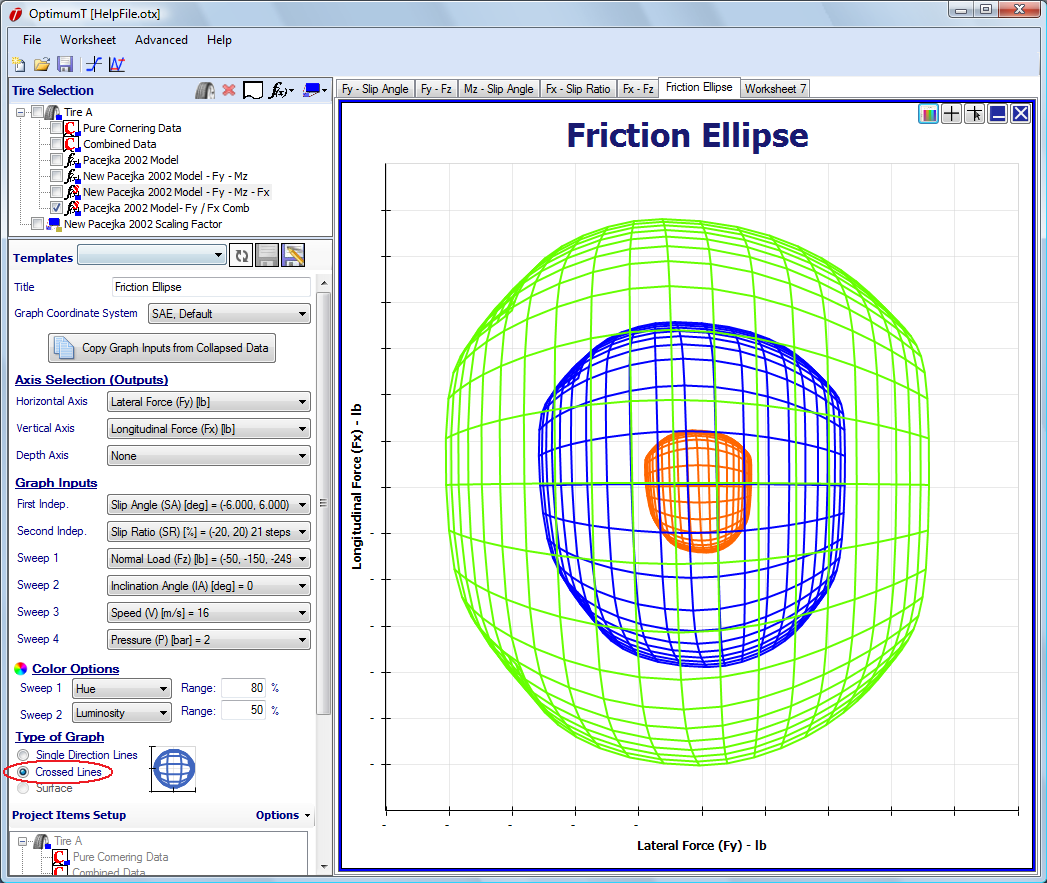
\includegraphics[width=1.0\textwidth]{CrossedLineGraph.png}
	\caption{Crossed Line Graph}
	\label{fig:CrossedLineGraph}
\end{figure}

\subsection*{Surface Graphs}
An example of a surface graph is shown in Figure~\ref{fig:SurfaceGraph}. Surface graphs are only available when a third graph output is selected in the Depth Axis drop down box. Surfaces are generated in the same way that crossed line plots are generated, but the area between the lines is filled to generate the surface.

\begin{figure}[H]
	\centering
		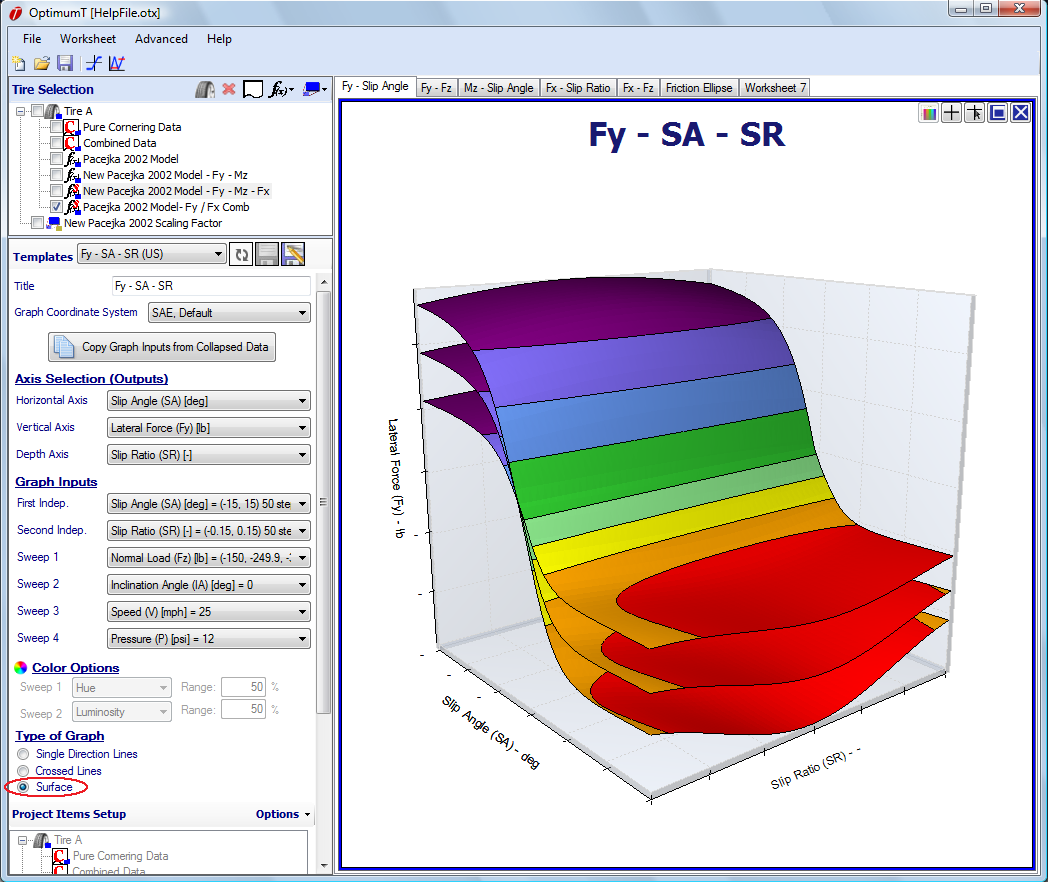
\includegraphics[width=1.0\textwidth]{SurfaceGraph.png}
	\caption{Surface Graph}
	\label{fig:SurfaceGraph}
\end{figure}

\subsection{Setting up a Standard Graph}
\label{sec:SettingupaStandardGraph}
For OptimumTire to generate a graph all six possible steady state tire conditions must be specified. These graph inputs are:

\begin{itemize}
\item Slip angle, $\alpha$
\item	Slip ratio, $\kappa$
\item	Normal load, $F_z$
\item	Inclination angle, $\gamma$
\item	Velocity, $V$
\item	Inflation pressure, $P$
\end{itemize}

In addition to the six graph inputs, the two graph outputs, the \textsl{Horizontal Axis} and \textsl{Vertical Axis} must be set to create a graph. If you are making a 3D graph a third output, the \textsl{Depth Axis}, must also be specified. Essentially, the OptimumTire plotting tool is evaluating a tire model or searching through the tire data for the three axes as follows:

	\begin{displaymath}
	 X=f_1(\alpha,\kappa,F_z,\gamma,V,P)
	\end{displaymath}
		\begin{displaymath}
	 Y=f_2(\alpha,\kappa,F_z,\gamma,V,P)
	\end{displaymath}
		\begin{displaymath}
	 Z=f_3(\alpha,\kappa,F_z,\gamma,V,P)
	\end{displaymath}

\subsection{Graph Outputs}
\label{sec:GraphOutputs}
The graph outputs specify what quantity and data range that each graph axis should represent. The graph output dialog is shown in Figure~\ref{fig:GraphOutput}. In this dialog the graph output to be used for each axis can be chosen. The unit displayed and the axis scaling can also be chosen. If the Auto Scale check box is selected, the scaling will adjust according to the data shown on the graph. The Auto Scale is unchecked then minimum and maximum value for the axis can be entered. Selecting Hide Axis Values will remove the numeric values from the graph axis. 

\begin{figure}[H]
	\centering
		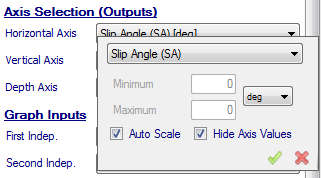
\includegraphics{GraphOutput.png}
	\caption{Graph Output Dialog}
	\label{fig:GraphOutput}
\end{figure}

Currently OptimumTire includes over 30 outputs that can be graphed. These outputs as well as their associated unit types are displayed in Table~\ref{tbl:GraphOutputs}. The unit types are displayed because OptimumTire allows the user to select between many different units. For more information about the available units in OptimumTire please refer to section~\ref{sec:Units}.

\begin{center}
\begin{longtable}{|c|c|}
			
			\hline
			\multicolumn{2}{|c|}{\cellcolor{tblue}\textbf{Graph Outputs}} \\ \hline
			\rowcolor{ttblue}\textbf{Basic} & \textbf{Unit Type} \\ \hline
			Inclination Angle (IA)	&angle \\ \hline
			Slip Angle (SA)	&angle \\ \hline
			Slip Ratio (SR)	&ratio \\ \hline
			Speed (V)	&velocity \\ \hline
			Pressure (P)	&pressure \\ \hline
			Loaded Radius (RL)	&length \\ \hline
			&\\ \hline
			
			\rowcolor{ttblue}\textbf{Force / Moment}	&\textbf{Unit Type} \\ \hline
			Longitudinal Force (Fx)	&force \\ \hline
			Lateral Force (Fy)	&force \\ \hline
			Normal Load (Fz)	&force \\ \hline
			Overturning  Moment (Mx)	&moment \\ \hline
			Rolling Resistance (My)	&moment \\ \hline
			Aligning Torque (Mz)	&moment \\ \hline
			&\\ \hline
						
			\rowcolor{ttblue}\textbf{Derivatives}	&\textbf{Unit Type} \\ \hline
			Cornering Stiffness 	&force / angle \\ \hline
			Inst. Cornering Stiffness 	&force / ratio \\ \hline
			Slip Stiffness	&force / angle \\ \hline
			Inst. Slip Stiffness	&force / ratio \\ \hline
			Camber Stiffness 	&force / angle \\ \hline
			Inst. Camber Stiffness	&force / angle \\ \hline
			Lateral Load Sensitivity & ratio \\ \hline
			Longitudinal Load Sensitivity &ratio \\ \hline
			Aligning Moment Load Sensitivity &length \\ \hline
			Overturning Moment Load Sensitivity &length \\ \hline
			Rolling Resistance Load Sensitivity &length \\ \hline
			 &\\ \hline
			
			\rowcolor{ttblue}\textbf{Normalized}	&\textbf{Unit Type} \\ \hline
			Normalized Longitudinal Force 	&ratio \\ \hline
			Normalized Lateral Force	&ratio \\ \hline
			Normalized Inst. Cornering Stiffness	&1 / angle \\ \hline
			Normalized Inst. Slip Stiffness	&ratio \\ \hline
			Normalized Inst. Camber Stiffness	&1 / angle \\ \hline
			Cornering Stiffness Coefficient	&1 / angle \\ \hline
			Slip Stiffness Coefficient	&ratio \\ \hline
			Camber Stiffness Coefficient	&1 / angle \\ \hline
			 &\\ \hline
			 
			\rowcolor{ttblue}\textbf{Coefficient of Friction}	&\textbf{Unit Type} \\ \hline
			Lateral Coefficient of Friction	&ratio \\ \hline
			Longitudinal Coefficient of Friction	&ratio \\ \hline
			 &\\ \hline
			 			
			\rowcolor{ttblue}\textbf{Moment Arm}	&\textbf{Unit Type} \\ \hline
			Pneumatic Trail	&length \\ \hline
			Pneumatic Scrub Radius	&length \\ \hline
			 &\\ \hline
			 
			\rowcolor{ttblue}\textbf{Peak}	&\textbf{Unit Type} \\ \hline
			Slip Angle at Peak Fy (negative)	&angle \\ \hline
			Slip Angle at Peak Fy (positive)	&angle \\ \hline
			Slip Ratio at Peak Fx (negative)	&ratio \\ \hline
			Slip Ratio at Peak Fx (positive)	&ratio \\ \hline
			Peak Lateral Force (negative)	&force \\ \hline
			Peak Lateral Force (positive)	&force \\ \hline
			Peak Longitudinal Force (negative)	&force \\ \hline
			Peak Longitudinal Force (positive)	&force \\ \hline
			 &\\ \hline
			 			
			\rowcolor{ttblue}\textbf{Offset}	&\textbf{Unit Type} \\ \hline
			Fx Offset (Fx @ SR = 0)	&force \\ \hline
			Fy Offset (Fy @ SA = 0)	&force \\ \hline
			 &\\ \hline
			
			\caption{Graph Outputs}
			\label{tbl:GraphOutputs}
\end{longtable}
\end{center}

\subsection{Graph Inputs}
\label{sec:GraphInputs}
The graph inputs can be \textsl{fixed values, constant sweeps} or \textsl{custom sweeps}. The graph inputs are specified by clicking on the box next to one of the six graph inputs.  A dialog box similar to that shown in Figure~\ref{fig:GraphInputs} will appear. The first item to be chosen is the variable for the graph input. This is chosen in the first dropdown box of the dialog. As can be seen in Figure~\ref{fig:GraphInputs} "Slip Angle" is currently selected as the first independent. As previously mentioned, all six inputs must be present.
 
For a \textsl{Single Line} graph the first graph input, labeled \textsl{Indep. Variable}, will be the quantity used to generate the graph lines. For a \textsl{Crossed Line} or \textsl{Surface graph} the first two graph inputs, labeled \textit{First Indep.} and \textit{Second Indep.}, will be the quantities used to generate the graph lines. The rest of the graph inputs, labeled \textsl{Sweep}, allow the plotting of multiple lines depending on the other tire conditions. For the first two of these, the option of changing the color of the graphed lines according to these inputs is available (see section~\ref{sec:ColoringGraphs} for more information).

The second dropdown box in this dialog allows the user to specify the type of sweep to be graphed. For each input in the graph input dialog three different types of sweeps can be chosen. The three sweep types available are: \textsl{Fixed Value}, \textsl{Constant Step Sweep}, and \textsl{Custom Sweep}. For the independent variables either the \textsl{Constant Step Sweep} or \textsl{Custom Sweep} should be used. For the sweep variables any of the sweep types can be used.

\begin{figure}[H]
	\centering
		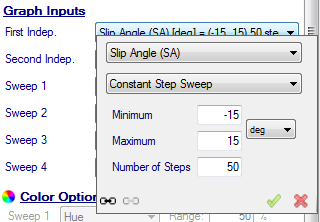
\includegraphics{GraphInputs.png}
	\caption{Graph Input Dialog}
	\label{fig:GraphInputs}
\end{figure}

\subsection*{Fixed Value Graph Inputs}
As the name suggests, fixed value graph inputs hold a particular variable constant when generating the graph. In the example shown in Figure~\ref{fig:FixedInput}, \textsl{Fixed} is selected in the second drop down box. Therefore the inclination angle is being held at a constant 2 degrees. In the fixed value dialog, there is also a box for data tolerance. This value tells OptimumTire what tolerance to use when searching raw data. Since there will always be some noise in the raw data, OptimumTire needs to know how far from the nominal value it should consider to be "close enough" to include in the plot.

\begin{figure}[H]
	\centering
		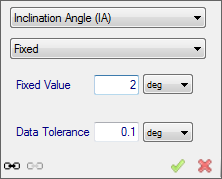
\includegraphics{FixedInput.png}
	\caption{Fixed Value Dialog}
	\label{fig:FixedInput}
\end{figure}

\subsection*{Constant Step Sweep Graph Inputs}
Constant step sweep graph inputs generate a set of evenly spaced points between a minimum and a maximum value. The constant sweep dialog is shown in Figure~\ref{fig:ConstantStepSweep}. A minimum and a maximum value for the sweep as well as the number of steps needs to be entered into the dialog. Constant sweep graph inputs do not have data tolerances as fixed graph inputs do. All data that falls within the specified range is used.

\begin{figure}[H]
	\centering
		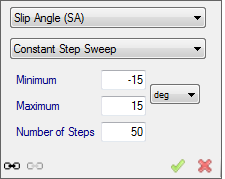
\includegraphics{ConstantStepSweep.png}
	\caption{Constant Step Sweep Dialog}
	\label{fig:ConstantStepSweep}
\end{figure}

\subsection*{Custom Sweep Graph Inputs}
A custom sweep graph input allows you to specify a number of arbitrary values. Figure~\ref{fig:CustomSweep} shows the custom sweep dialog. You can specify any number of values by typing them into the table. Additional rows can be added by clicking on the green "+" and rows can be removed by clicking on the red "-" above the input list. Like the fixed value graph input, custom sweep graph inputs have data tolerances.

\begin{figure}[H]
	\centering
		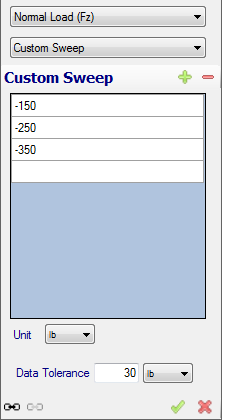
\includegraphics{CustomSweep.png}
	\caption{Custom Sweep Dialog}
	\label{fig:CustomSweep}
\end{figure}

\subsection{Plotting Raw Data}
\label{sec:PlottingRawData}
Initially when raw data is imported and graphed in OptimumTire all of the data will be plotted regardless of the graph input parameters. This \textsl{Plot all Data} feature allows the user to quickly view data to ensure that it is the correct data and that it was imported successfully. If the user would like to graph data at certain conditions specified by the graph inputs, this feature needs to be unselected.

When the \textsl{Plot all Data} option is unselected, OptimumTire will search for raw data points that correspond to all six of the graph inputs. Points matching the six conditions will be plotted on the graph. 

There are three different ways to unselect the \textsl{Plot All Data}. The first one is by right clicking on the raw data in the project tree and selecting Remove \textsl{"Plot All Data"} In \textsl{All Graphs}. This is shown in Figure~\ref{fig:ProjectTreePlotAllData}. This will disable the feature for the selected data set in all of the graphs.

\begin{figure}[H]
	\centering
		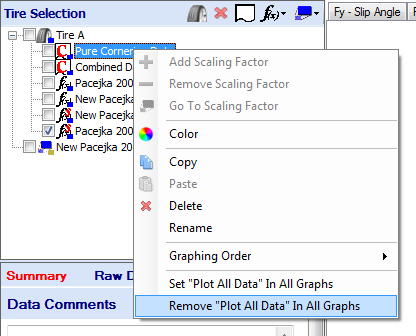
\includegraphics{ProjectTreePlotAllData.png}
	\caption{Plot All Data Option in Project Tree}
	\label{fig:ProjectTreePlotAllData}
\end{figure}

The other two procedures to unselect this option are located in the \textsl{Project Items Setup} at the bottom of the graph setup form as shown in Figure~\ref{fig:ProjectItemSetup}. Since this is located in the graph setup form it will only affect the graph that it corresponds to. As can be seen \textsl{"<all data>"} will appear to the right of the name of the data if \textsl{Plot All Data} is enabled. By right clicking on the data and clicking on the Plot All Data selects or unselects this feature. The \textsl{Options} button in the upper right of the figure allows the user to set all or no items to \textsl{Plot All Data}. Again this will change all of the items for the current graph only. 

\begin{figure}[H]
	\centering
		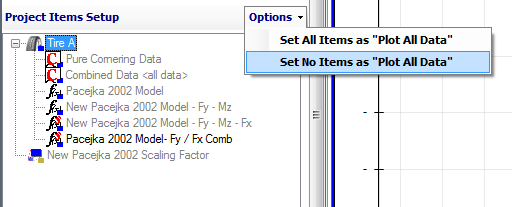
\includegraphics[width=1.0\textwidth]{ProjectItemSetup.png}
	\caption{Project Item Setup}
	\label{fig:ProjectItemSetup}
\end{figure}

\subsection{Copy Graph Inputs from Collapsed Data}
\label{sec:CopyGraphInputsfromCollapsedData}
The \textsl{Copy Inputs from Collapsed Data} button located on the graph setup form is shown in Figure~\ref{fig:CopyFromCollapsedButton}.   This feature allows the user to quickly set the graph inputs. It will copy the values and tolerances set in the data collapsing into the graph setup inputs. Therefore to use this feature the current project must contain collapsed data.

\begin{figure}[H]
	\centering
		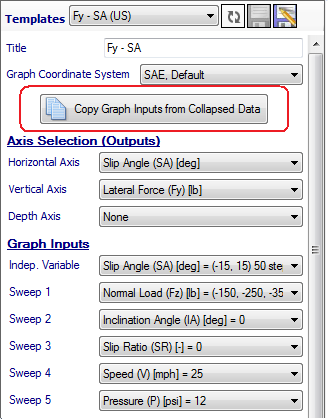
\includegraphics{CopyFromCollapsedButton.png}
	\caption{Copy Inputs from Collapsed Data Button}
	\label{fig:CopyFromCollapsedButton}
\end{figure}

When this button is clicked a window similar to the one shown in Figure~\ref{fig:CopyFromCollapsed} will appear. This window displays all of the collapsed data in the project. Selecting one of the data sets and pressing the \textsl{Copy} button will import the collapsed data values and tolerances into the graph setup form, therefore instantly plotting the data at all of its tested conditions.

\begin{figure}[H]
	\centering
		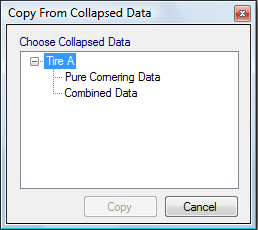
\includegraphics{CopyFromCollapsed.png}
	\caption{Copy Inputs from Collapsed Data Window}
	\label{fig:CopyFromCollapsed}
\end{figure}

\subsection{Linking Graphs}
\label{sec:LinkingGraphs}
The data input in different graphs can be linked together. Thus when the linked input in one of the graphs is changed it will be applied to the other graphs that are linked to it. The inputs are linked by clicking on the \textsl{Link Sweep} button. This button as well as the \textsl{Unlink Sweep} button is circled in Figure~\ref{fig:LinkGraphs}. After clicking on this button a message box that says \textsl{Please select a graph} will appear. Clicking on any of the other graphs will link them to the original graph. The linked input of the original graph will now change to reflect the input of the selected graph. If you would like to link another graph to these two, click the \textsl{Link Sweep} button on that graph and then choose one of the previously linked graphs. Multiple graphs and inputs can be linked together in the same fashion.

\begin{figure}[H]
	\centering
		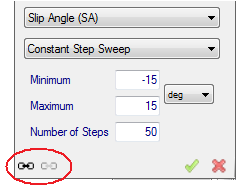
\includegraphics{LinkGraphs.png}
	\caption{Linking Graphs}
	\label{fig:LinkGraphs}
\end{figure}

\subsection{Coloring Graphs}
\label{sec:ColoringGraphs}
The color of the graphs is based on the color assigned to the project item. This can be changed by right-clicking on the item in the project tree and selecting \textsl{color}. Then a window will open were the user can choose the base color to be used. This will change the color of the item in all of the graphs. The color of all of the items in one tire can also be changed. This is done by right clicking on the tire itself and selecting \textsl{color}.  The color in the bottom right corner of the item icon displays the current base color of that item.

The base color of an item can also be changed in each graph separately. This can be done in the \textsl{Project Items Setup} at the bottom of the graph setup form. By right clicking on an item in this list the user is given the option to \textsl{Set Custom Color or Return to Default Color}. Selecting Set \textsl{Custom Color} will allow the user to change the base color of this item in only the current graph. \textsl{Selecting Return to Default Color} will change the color to the color of the same item in the project tree. 

\begin{figure}[H]
	\centering
		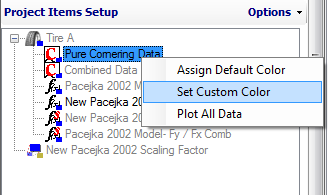
\includegraphics{CustomColor.png}
	\caption{Plot All Data Option}
	\label{fig:CustomColor}
\end{figure}

If you choose, you can also alter the color of the graph based on two of the graph inputs. This will modify the base color depending on the first two input sweeps of the graph. The color of the data sweeps can be altered in the bottom of the graph input form as seen in Figure~\ref{fig:ColorOptions}. The color is altered according to the color quantity selected. These include \textsl{Constant Color}, \textsl{Hue}, \textsl{Luminosity,} or \textsl{Saturation}. 

\begin{figure}[H]
	\centering
		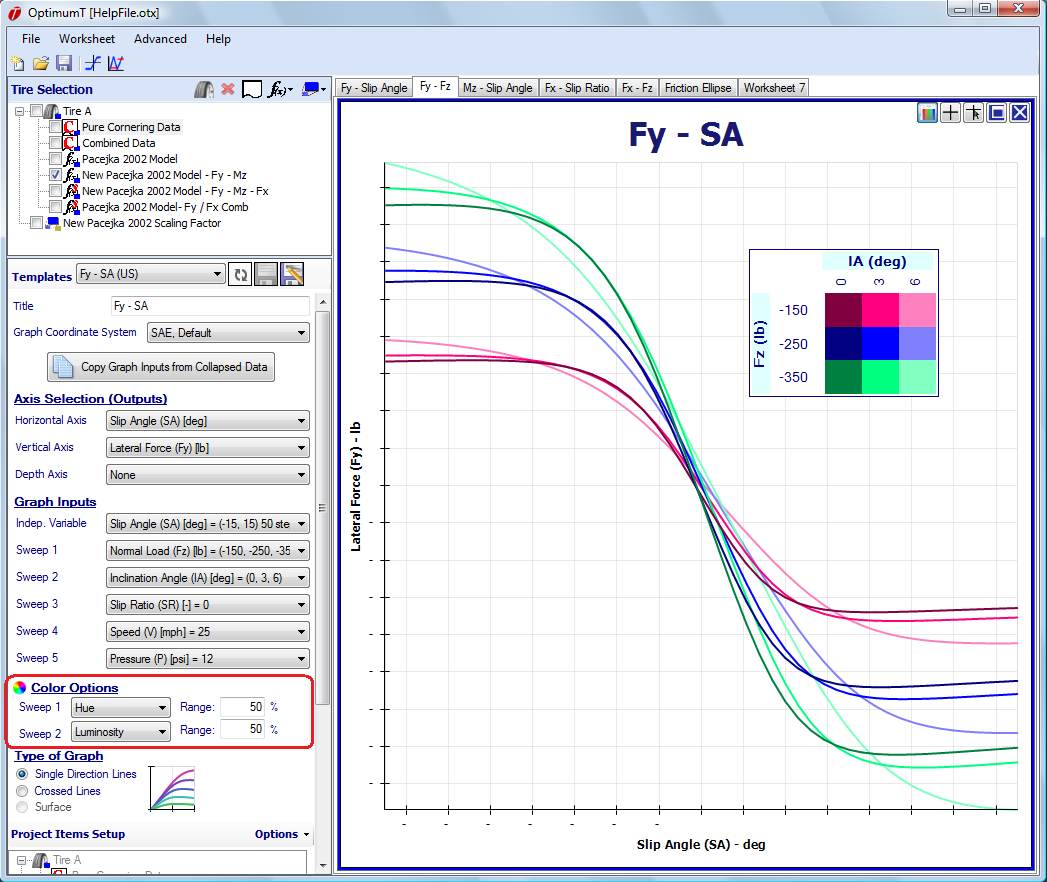
\includegraphics[width=1.0\textwidth]{ColorOptions.png}
	\caption{Color Setup}
	\label{fig:ColorOptions}
\end{figure}

Hue will change the actual color of the lines according to the input sweeps as shown in Figure~\ref{fig:Hue}. Luminosity will affect the visibility of the lines as shown in Figure~\ref{fig:Luminosity} and Saturation will affect the brightness of the lines as shown in Figure~\ref{fig:Saturation}.  In Figure~\ref{fig:ColorOptions} hue is varied with the vertical load and the luminosity is varied with the inclination angle. The range for these quantities in percentage can be entered in the textboxes to the right. A higher range will create a larger difference in color between the lines. Custom coloring is not currently available for the surface graphs.

\begin{figure}[H]
	\centering
		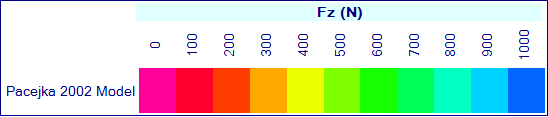
\includegraphics[width=1.0\textwidth]{Hue.png}
	\caption{Hue}
	\label{fig:Hue}
\end{figure}

\begin{figure}[H]
	\centering
		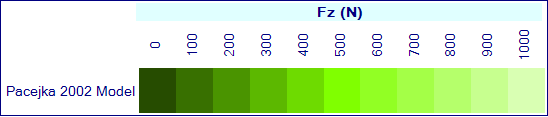
\includegraphics[width=1.0\textwidth]{Luminosity.png}
	\caption{Luminosity}
	\label{fig:Luminosity}
\end{figure}

\begin{figure}[H]
	\centering
		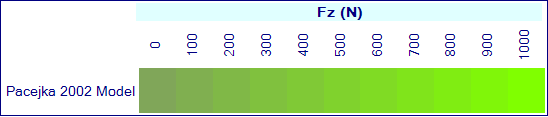
\includegraphics[width=1.0\textwidth]{Saturation.png}
	\caption{Saturation}
	\label{fig:Saturation}
\end{figure}

\subsection{Graph Templates}
\label{sec:GraphTemplates}
Graph templates allow the user to quickly display commonly used graphs. They can be accessed at the top of the graph setup form as shown in Figure 4.19.Graph templates in the predefined folder are supplied with OptimumTire. These templates cannot directly be modified but can be changed and saved as new templates. They also can be copied into the user folder in the template manager.

\begin{figure}[H]
	\centering
		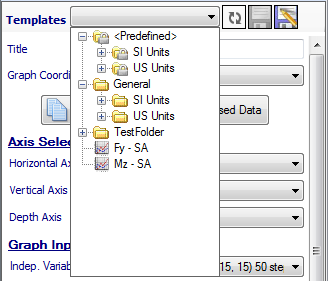
\includegraphics{GraphTemplates.png}
	\caption{Graph Templates}
	\label{fig:GraphTemplates}
\end{figure}

To load a graph template, select it from the list and click the Load Graph Template button (which will be spinning after you choose a template). To save a new template, click on the save-as button next to the graph template list. Clicking the save button when a graph template is selected will overwrite the selected graph template.

\section{Report Graphs}
\label{sec:ReportGraphs}
Report graphs display data versus sample number (which is proportional to time). Only raw tire data can be shown on report graphs. An example of a report graph is shown in Figure~\ref{fig:ReportGraph}. This is the same type of graph that is used in the data cropping tool. When this graph is selected a report graph setup form will appear in the data entry area. At the top of the form a title can be added to the graph and the coordinate system that the data will be displayed in can be changed. The quantities to be graphed (i.e slip angle) can be selected from the checkboxes in this form. Multiple quantities can be graphed at the same time. At the bottom of the form the user can set the axis parameters including the minimum and maximum range (or Auto Scale) and the display units.
 
By clicking on the graph, the data cursor (vertical black line) can be moved. The data values to the right of the graph quantities in the setup form represent the values of the data at the data cursor location. The graph can be zoomed in and out with the middle mouse button. While holding down the middle mouse button, draw a box from the top left to the bottom right corner of the area you want to zoom in on. Drawing a box in the opposite direction will un-zoom the graph. Right clicking on the mouse gives the user options to copy or print the graph as well add additional graphs or worksheets to the project.


\begin{figure}[H]
	\centering
		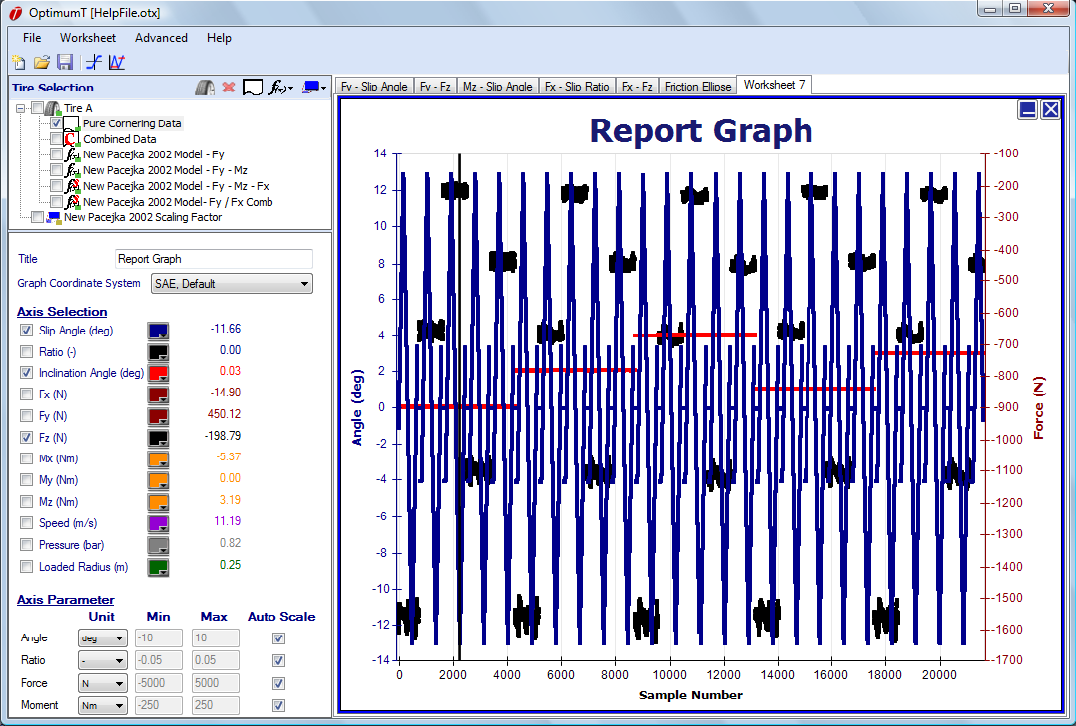
\includegraphics[width=1.0\textwidth]{ReportGraph.png}
	\caption{Report Graph}
	\label{fig:ReportGraph}
\end{figure}

\section{Graph Area Options}
\label{sec:GraphAreaOptions}
In the upper right corner of each standard graph there are buttons that allow the user to access additional graphing options. These buttons are shown in Figure~\ref{fig:GraphAreaOptionsLabeled}. The two buttons on the far right are similar to typical windows buttons. The one on the far right will permanently close the graph and the other one will minimize or maximize the graph depending on its current state. The other three buttons are custom options in OptimumTire. These will first be discussed in detail in this section and then other graph options that can be accessed by right clicking on the graph will be covered.

\begin{figure}[H]
	\centering
		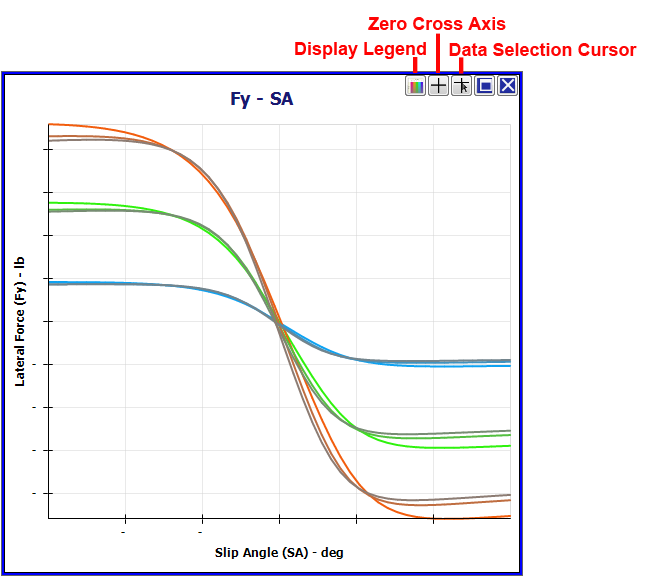
\includegraphics[width=1.0\textwidth]{GraphAreaOptionsLabeled.png}
	\caption{Graph Area Options}
	\label{fig:GraphAreaOptionsLabeled}
\end{figure}

\subsection{Display Legend}
\label{sec:DisplayLegend}
The \textsl{Display Legend} button on the far left allows the user to show the graph legend. Clicking on this button will display the legend as shown below in Figure~\ref{fig:GraphLegend}. The legend can be moved by holding down the mouse button on it and dragging it to the desired location. It can also be resized by holding the mouse button down on the corners of the legend and dragging it to the desired size.

\begin{figure}[H]
	\centering
		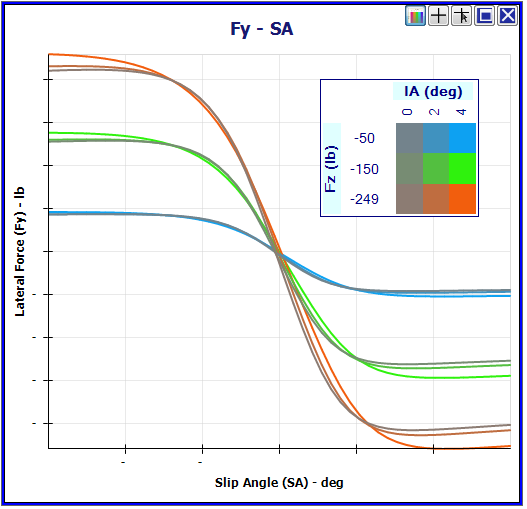
\includegraphics[width=1.0\textwidth]{GraphLegend.png}
	\caption{Graph Legend for two Data Sweeps}
	\label{fig:GraphLegend}
\end{figure}

In Figure~\ref{fig:GraphLegend} the legend displays the values and colors corresponding to the inputs in Sweep 1 and Sweep 2 in the graph setup form. Since both inputs were set as sweeps both are displayed in the legend.

If neither or only one of the first two graph inputs include multiple values, the legend will display the names of the items in the project tree that are being graphed. This is shown below in Figure \ref{fig:OverrideLegendName}.

\begin{figure}[H]
	\centering
		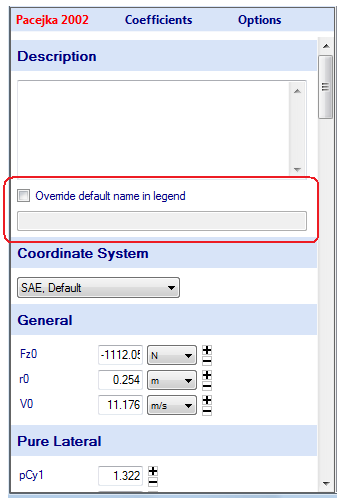
\includegraphics{OverrideLegendName.png}
	\caption{Graph Legend for one Data Sweep}
	\label{fig:OverrideLegendName}
\end{figure}

The names displayed in the legend can also be modified in the data entry area corresponding to the selected Item. Therefore to change the legend name without renaming the item, click on the item in the project tree. Then the form shown in Figure~\ref{fig:OverrideLegendName} will appear in the data entry area.  Selecting or deselecting the checkbox labeled \textsl{Override the default name in legend} will change the name of the item shown in the legend. When it is checked whatever text is entered into the textbox below the checkbox will appear in the legend instead of the name of the item.

\subsection{Axis Zero Cross}
\label{sec:AxisZeroCross}
The \textsl{Axis Zero Cross} button is the second button from the left. By default the graph axis will be displayed at the borders of the graph. When this button is selected the axis will be displayed on the gridlines corresponding to the zero value of the graph outputs. This is shown in Figure~\ref{fig:ZeroCross}.

\begin{figure}[H]
	\centering
		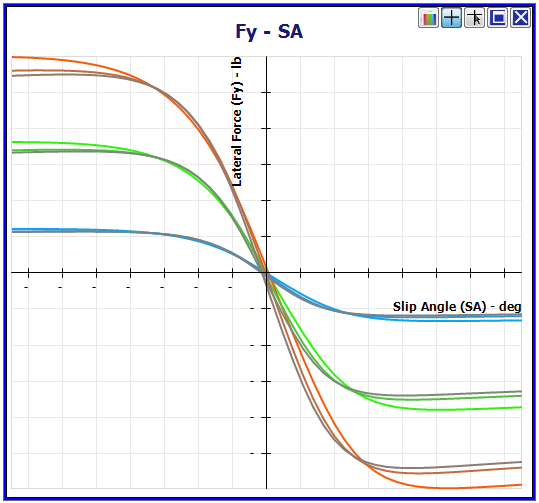
\includegraphics[width=1.0\textwidth]{ZeroCross.png}
	\caption{Zero Cross Axis}
	\label{fig:ZeroCross}
\end{figure}

\subsection{Data Selection Cursor}
\label{sec:DataSelectionCursor}
The \textsl{Data Selection Cursor} allows the user to easily and quickly get information about a specific data point or line. An example of this is shown in Figure~\ref{fig:DataSelection}.   After clicking on the \textsl{Data Selection Cursor} button, click on either a data line or point in the graph to see the test conditions and values corresponding to that specific location.

\begin{figure}[H]
	\centering
		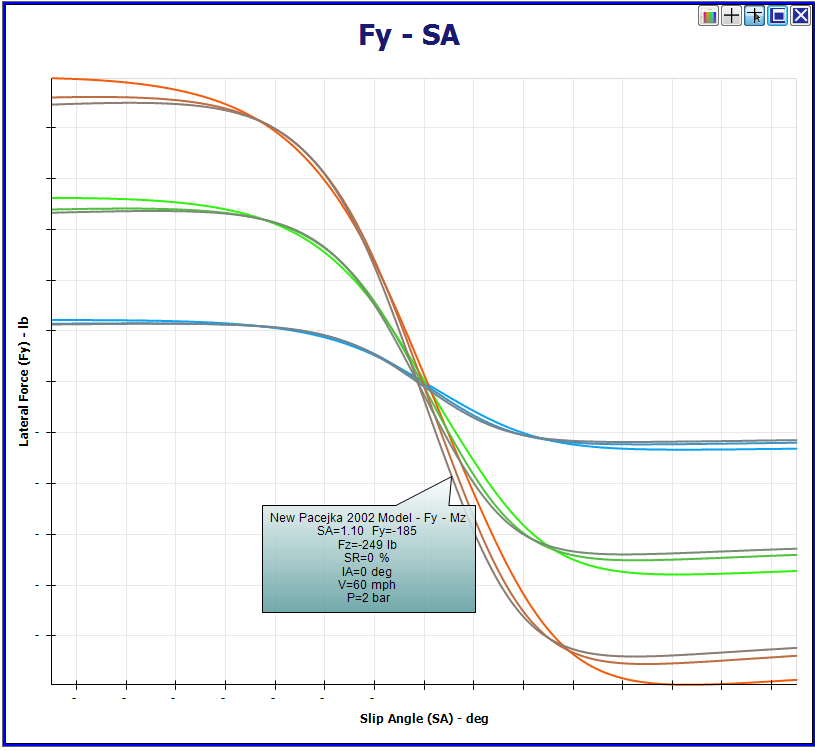
\includegraphics[width=1.0\textwidth]{DataSelection.png}
	\caption{Data Cursor Selection}
	\label{fig:DataSelection}
\end{figure}

\subsection{Copy and Print Graphs}
\label{sec:CopyandPrintGraphs}
Graphs can be easily copied or printed from OptimumTire.  These options are available through right clicking on either a standard or report graph as shown in Figure~\ref{fig:RightClickOptions}. If \textsl{Copy graph to Clipboard} is selected than an image of the current graph will be copied to the windows clipboard. The user can then paste this image into other programs. If \textsl{Print Graph} is selected the standard printing options window will open allowing the user to select the printer and set the printing preferences. When printed the graph will be automatically resized and centered to fit on a standard 8.5" x 11" piece of paper.

\begin{figure}[H]
	\centering
		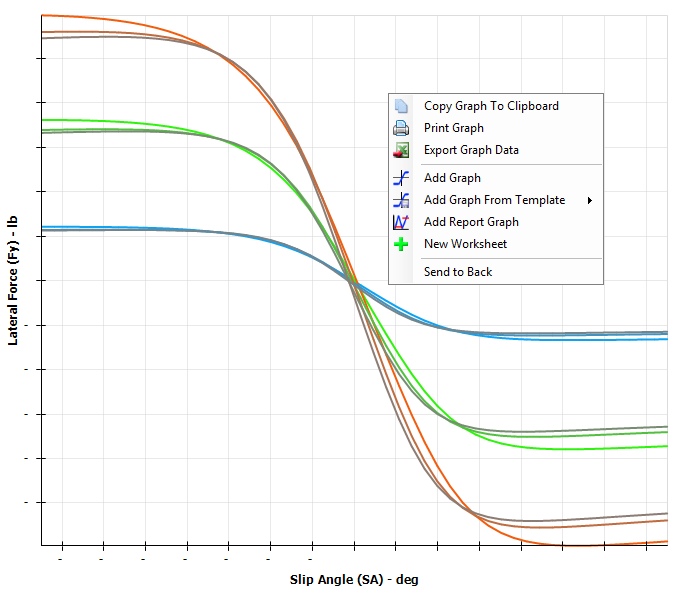
\includegraphics[width=1.0\textwidth]{RightClickOptions.png}
	\caption{Right Click Options}
	\label{fig:RightClickOptions}
\end{figure}

\subsection{Export Graph Data}
\label{sec:ExportGraphData}
Another feature shown in Figure~\ref{fig:RightClickOptions} is the Export Graph Data. When this is selected the data that is currently plotted will be exported and saved to an Excel file. The different data sweeps will be separated by different headers indicating the conditions that they represent. An example of this is shown in Figure~\ref{fig:ExcelExport}.

\begin{figure}[H]
	\centering
		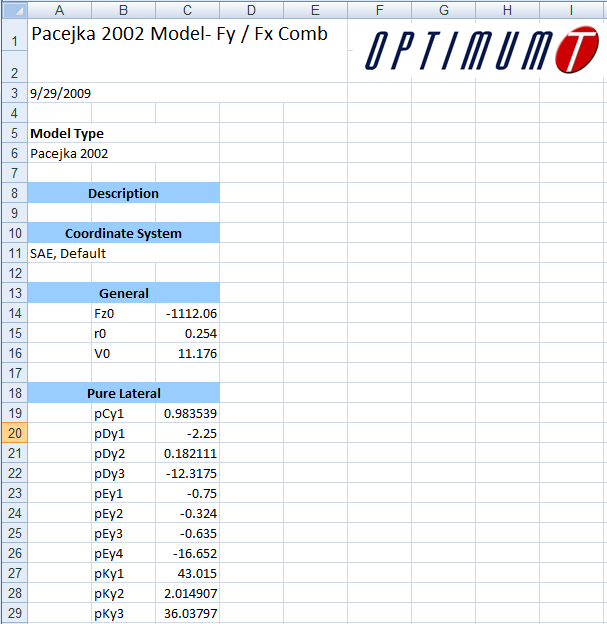
\includegraphics[width=1.0\textwidth]{ExcelExport.png}
	\caption{Excel Export Format}
	\label{fig:ExcelExport}
\end{figure}
